\documentclass[sigconf]{acmart}

\AtBeginDocument{%
  \providecommand\BibTeX{{%
    \normalfont B\kern-0.5em{\scshape i\kern-0.25em b}\kern-0.8em\TeX}}}

\usepackage{dblfloatfix}
\usepackage{mathtools}
\usepackage{hyperref}
\usepackage[htt]{hyphenat}

\begin{document}

\title{Information retrieval and Text Mining : Group Project}

% AUTHORS:
\author{Til Mohr}
\affiliation{}
\email{tv.mohr@stud.uis.no}

\author{Ishaac Ourahou}
\affiliation{}
\email{i.ourahou@stud.uis.no}

% DATE:
\date{\today}



\begin{abstract}
In our master's degree program, we delved into the realms of information retrieval and text mining. Our group project focuses on developing a system capable of searching for specific passages within a conversation. This entails considering the historical context of previous exchanges when interpreting the current user's query. The system reformulates the user's query to better align with the conversation's overarching topic and then seeks the most relevant passages from a vast collection of 8.8 million documents, specifically from the MS MARCO document collection. We initially create a baseline information retrieval pipeline, which serves as our foundational reference. We then explore advanced techniques and methods in the field of conversational search engines. Our report concludes with a comparative analysis between the baseline system and our advanced retrieval mechanisms, outlining the strengths and shortcomings of our approaches, and offering conclusions.
\end{abstract}

\keywords{information retrieval, conversational search engine, conversational search system}

%% Remove copyright footer
\settopmatter{printacmref=false}
\setcopyright{none}
\renewcommand\footnotetextcopyrightpermission[1]{}
\pagestyle{plain}
%% ------------------------

%%
%% This command processes the author and affiliation and title
%% information and builds the first part of the formatted document.
\maketitle


\section{Introduction}\label{sec:intro}
With the rise of conversational agents like Amazon Alexa and Apple Siri, the ability to accurately and relevantly respond to user requests has become increasingly important. These agents are designed to interact fluidly with users, and the essence of their functionality rests on providing precise information in their responses.

Our project centers on building a conversational search engine, a system that not only addresses the user's immediate question but also takes into account previous queries and the ongoing conversation's topic. This provides a more holistic approach to the user's information needs. Initially, we will construct a basic architecture, establishing our baseline system. This baseline will serve as a comparison point against more sophisticated techniques. It's required, however, that even this foundational system meets or exceeds the performance of the reference system set by our project guides.

Our research will utilize the MS MARCO dataset, a comprehensive collection of 8.8 million documents. Efficiently retrieving relevant documents from this vast pool necessitates an indexing process, which we will execute using the \texttt{pyterrier} API.

Section \ref{sec:problem} will articulate the specific problem we aim to address. We will then elaborate on the methodologies behind our retrieval pipelines. Broadly, these pipelines can be broken down into stages: Query revision, single- or multi-pass retrieval, and reranking. Sections \ref{sec:baseline} and \ref{sec:advanced} will delve into our baseline and advanced techniques for each of these stages, respectively. Our report will conclude in section \ref{sec:results}, where we evaluate and compare the effectiveness of our systems, highlighting the strengths and potential areas of enhancement in our advanced approaches.

The codebase for our project can be found on GitHub\footnote{URL: \url{https://github.com/CodingTil/2023_24---IRTM---Group-Project}}.

\section{Problem Statement}\label{sec:problem}
This project focuses on developing a Conversational Search Engine (CSE). What distinguishes a CSE from a traditional search engine is its inherent context-aware nature. In a CSE, queries asked by a user within a session are semantically interconnected. Rather than treating each query in isolation, a CSE leverages information from both the previous queries and the system's responses to those queries to retrieve relevant passages. It must cater to the continuous thread of a dialogue, while also being agile enough to accommodate sudden shifts in conversation topics. For every user query, the goal is to generate a ranked listing of the top 1000 passages out of an expansive 8.8 million document collection.

A vital component that sets a CSE apart is its query rewriting mechanism. This feature reformulates the presented query to better reflect the ongoing conversation topic. Figure \ref{figure:global_pipeline} offers a schematic representation of how the various stages of a CSE retrieval pipeline interact. Analogous to traditional search engines, a CSE also requires prior indexing of the document collection, enabling computationally efficient retrieval and ranking processes.

\begin{figure}[h]
	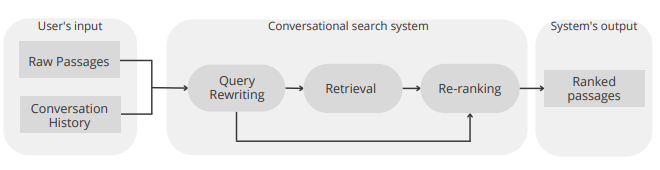
\includegraphics[width=7cm]{pipeline.png}
	\caption{Overall system's pipeline architecture}
	\label{figure:global_pipeline}
\end{figure}


\section{Baseline Method}\label{sec:baseline}
Our baseline method is inspired by the baseline method presented by Łajewska et al. \cite{Lajewska:2023:ECIR}. Our baseline method is structured in the following sequence:
\begin{enumerate}
	\item	\texttt{T5} Query Rewriting
	\item	\texttt{BM25} Retrieval
	\item	Re-ranking
			\begin{enumerate}
				\item	Re-ranking using \texttt{monoT5}
				\item	Top-document re-ranking using \texttt{duoT5}
			\end{enumerate}
\end{enumerate}

\subsection{T5 Query Rewriting}
In conversation search engines, query rewriting is the crucial component to include the semantics of the conversation history into the currently asked query, which results into a singular rewritten query that can be fed into the retrieval pipeline.

For this purpose, we include all the previously rewritten queries $q'_0 \dots q'_{n-1}$ of our conversation, as well as the response $r_{n-1}$ of the CSE to the previous rewritten query $q'_{n-1}$ into the current query $q_n$. This is done by concatenating the previous rewritten queries and the response into a single string:
\begin{align*}
	q'_n \coloneqq q'_0 \text{<sep>} \dots \text{<sep>} q'_{n-1} \text{<sep>} r_{n-1} \text{<sep>} q_n
\end{align*}
This approach resembles the approach taken by Łajewska et al. \cite{Lajewska:2023:ECIR}.

We have found through experimentation that this mere concatenation is insufficient to produce satisfiable results: The concatenated string is too long, and too much focus during the later retrieval is being put on $r_{n-1}$, which make responses sudden topic changes impossible.

Driven by these insights, we have turned our attention to other query rewriting techniques. \texttt{Pyterrier} provides the \texttt{SequentialDependence} query rewriting method\footnote{URL: \url{https://pyterrier.readthedocs.io/en/latest/rewrite.html\#sequentialdependence}}. We have found, however, that this rewriter also does not produce the desired results.

Subsequent exploration led us to the \texttt{T5} neural query rewriter trained for conversational question rewriting\footnote{URL: \url{https://huggingface.co/castorini/t5-base-canard}}. With this method, $q'_n$ closely mirrored $q_n$, subtly infusing it with the conversation's context, particularly when no drastic topic alterations were identified. A valuable by-product was the concise nature of the rewritten query, a departure from the growing length observed previously.

\subsection{BM25 Retrieval}
We settled on the \texttt{BM25} retrieval method, a commonly used formula in the realm of information retrieval, for its simplicity and its deployment in the reference system, allowing for direct comparisons.

\subsection{Re-ranking}
The re-ranking stage of our baseline system consists of two stages: First, the top 1000 documents retrieved by the \texttt{BM25} retrieval method are re-ranked using the \texttt{monoT5} reranker. Afterwards, the top 50 documents of the previous re-ranking stage are rearranged using the \texttt{duoT5} reranker. e precise count of documents subject to reranking at each stage is a hyperparameter of our system, allowing to balance computational cost and result quality. These rerankers were implemented in the \texttt{pyterrier\_t5} library.\footnote{URL: \url{https://github.com/terrierteam/pyterrier_t5}}


\section{Advanced Method}\label{sec:advanced}
Explain what you are taking as your advanced method(s), as well as why this is a promising attempt to outperform the baseline method, and why you are making specific implementation choices.

\section{Results}\label{sec:results}
The individual methods were evaluated on the MS MARCO document collection and the following provided files: \texttt{queries\_train.csv}, comprising of a list of queries grouped together into several conversation sessions, and \texttt{qrels\_train.txt} that contains the relevance assessments for the training queries. Our evaluation focused on a suite of metrics:
\begin{itemize}
	\item	Recall at 1000 (R@1000)
	\item	Mean Average Precision (MAP)
	\item	Mean Reciprocal Rank (MRR)
	\item	Normalized Discounted Cumulative Gain (NDCG\_Cut@3)
\end{itemize}
These metrics were calculated using the \texttt{trec\_eval} tool:
\begin{verbatim}
trec_eval -c -m recall.1000 -m map -m recip_rank
-m ndcg_cut.3 -l2 -M1000 qrels_train.txt
{GENERATED_TREC_RUNFILE}
\end{verbatim}

As stated in section \ref{sec:baseline}, the baseline method can be parameterized in a few different ways. For this evaluation, we utilized the following configurations: The document retrieval (\texttt{BM25}) used the default parameters from \texttt{pyterrier}\footnote{URL: \url{https://pyterrier.readthedocs.io/en/latest/terrier-retrieval.html}} to retrieve the 1000 most-relevant documents for each query. All 1000 documents were then reranked using the \texttt{monoT5} reranker. Because of the high computational cost of the \texttt{duoT5} reranker, only of those 1000 documents the best 50 documents were then reordered using this reranker.

\begin{table}[h]
\begin{center}
	\caption{Performance of the different methods on the MS MARCO document collection.}
	\begin{tabular}{l|rrrr}
			& R@1000 & MAP & MRR & NDCG\_Cut@3 \\
		\hline
		Reference System & ??? & ??? & ??? & ??? \\
		Baseline Method & $0.1746$ & $0.3230$ & $0.5705$ & $0.2461$ \\
	\end{tabular}
	\label{table:1}
\end{center}
\end{table}

\section{Discussion and Conclusions}

Summarize and discuss different challenges you faced and how you solved those. Include interpretations of the key facts and trends you observed and pointed out in the Results section. Which method performed best, and why? Speculate: What could you have done differently, and what consequences would that have had?

%%
%% If your work has an appendix, this is the place to put it.
%\appendix

%\section{Appendix}


%%
%% The next two lines define the bibliography style to be used, and
%% the bibliography file.
\bibliographystyle{ACM-Reference-Format}
\bibliography{main}

\newpage
\appendix
\section{Division of Work During the Project}

\end{document}
\endinput
